%
% primitiv.tex -- slide template
%
% (c) 2021 Prof Dr Andreas Müller, OST Ostschweizer Fachhochschule
%
\bgroup
\begin{frame}[t]
\setlength{\abovedisplayskip}{5pt}
\setlength{\belowdisplayskip}{5pt}
\frametitle{Primitive Matrix}
\vspace{-20pt}
\begin{columns}[t,onlytextwidth]
\begin{column}{0.48\textwidth}
\begin{block}{Definition}
$A\ge 0$ heisst primitiv, wenn es ein $n>0$ gibt mit $A^n>0$
\end{block}
\uncover<9->{%
\begin{block}{Intuition}
\begin{itemize}
\item<10->
Markov-Ketten: $a_{ij} > 0$ bedeutet, $i$ von $j$ aus erreichbar.
\item<11->
Band: {\em alle} Verbindung mit allen Nachbarn
\item<12->
$n$-te Potenz: Pfade der Länge $n$ 
\item<13->
Durchmesser: wenn $n>\text{Durchmesser des Zustandsdiagramms}$,
dann ist $A^n>0$
\end{itemize}
\end{block}
}
\end{column}
\begin{column}{0.48\textwidth}
\uncover<2->{%
\begin{block}{Beispiel: Reduzible W'keitsmatrix}
\vspace{-5pt}
\begin{center}
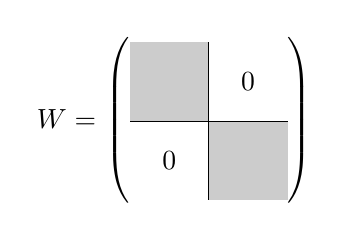
\begin{tikzpicture}[>=latex,thick]
\fill[color=gray!40] (-1,0) rectangle (0,1);
\fill[color=gray!40] (0,-1) rectangle (1,0);
\draw[line width=0.3pt] (0,-1) -- (0,1);
\draw[line width=0.3pt] (-1,0) -- (1,0);
%\draw (-1,-1) rectangle (1,1);
\node at (0,0) {$\left( \raisebox{0pt}[1cm][1cm]{\hspace*{2cm}} \right)$};
\node at (-1.3,0) [left] {$\mathstrut W=$};
\node at (0.5,0.5) {$0$};
\node at (-0.5,-0.5) {$0$};
\end{tikzpicture}
\end{center}
\vspace{-10pt}

$\Rightarrow$ $W$ ist nicht primitiv
\end{block}}
\uncover<3->{%
\begin{block}{Beispiel: Bandmatrix}
\centering
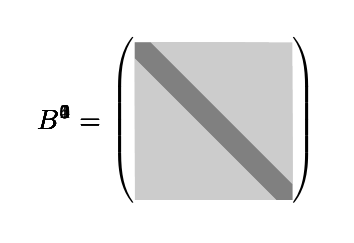
\begin{tikzpicture}[>=latex,thick]
\begin{scope}
\clip (-1,-1) rectangle (1,1);
\foreach \n in {3,...,8}{
	\pgfmathparse{0.3*(\n-2)}
	\xdef\x{\pgfmathresult}
	\only<\n>{
		\fill[color=gray!40]
			({-1.2-\x},1) -- (1,{-1.2-\x}) -- (1,{-0.8+\x})
			-- ({-0.8+\x},1) -- cycle;
	}
}
\fill[color=gray] (-1.2,1) -- (1,-1.2) -- (1,-0.8) -- (-0.8,1) -- cycle;
\end{scope}
\foreach \n in {2,...,8}{
	\uncover<\n>{
		\pgfmathparse{int(\n-2)}
		\xdef\k{\pgfmathresult}
		\node at (-1.3,0) [left] {$\mathstrut B^{\k}=$};
	}
}
\node at (0,0) {$\left( \raisebox{0pt}[1cm][1cm]{\hspace*{2cm}} \right)$};
\end{tikzpicture}
\end{block}}
\end{column}
\end{columns}
\end{frame}
\egroup
